\documentclass[letterpaper,10pt,conference]{ieeeconf}

\IEEEoverridecommandlockouts
\overrideIEEEmargins

\usepackage{graphicx}
\graphicspath{{./}{../}}
\usepackage{amsmath,amssymb}
\usepackage{cite}
\usepackage{booktabs}
\usepackage{multirow}
\usepackage{microtype}
\usepackage{xcolor}
\usepackage{xspace}
\usepackage{placeins}
\usepackage{balance}
\usepackage{url}
\usepackage[hidelinks]{hyperref}

\newcommand{\method}{LOGIV\xspace}
\newcommand{\T}{\textsc{true}}
\newcommand{\F}{\textsc{false}}
\newcommand{\U}{\textsc{unresolved}}
\definecolor{algcommentblue}{RGB}{0,125,155}
\newcounter{algorithm}
\newcounter{algline}
\newenvironment{algorithm}[1][t]{%
  \begin{figure}[#1]\refstepcounter{algorithm}\footnotesize
}{\end{figure}}
\newcommand{\algcaption}[1]{%
  \noindent\textbf{Algorithm~\thealgorithm\quad #1}\par\vspace{3pt}\hrule\vspace{4pt}}
\newenvironment{compactalgorithmic}{%
  \begin{list}{\arabic{algline}}{%
    \usecounter{algline}
    \setlength{\leftmargin}{1.55em}
    \setlength{\labelwidth}{1.05em}
    \setlength{\labelsep}{0.45em}
    \setlength{\itemsep}{0.8pt}
    \setlength{\parsep}{0pt}
    \setlength{\topsep}{3pt}
    \setlength{\partopsep}{0pt}}
}{\end{list}}
\newcommand{\algcomment}[1]{{\color{algcommentblue}// #1}}

\title{LOGIV: Graph-Verified Execution with Causal Local Repair for Long-Horizon Robot Tasks}
\author{Anonymous Authors}

\begin{document}
\maketitle
\thispagestyle{empty}
\pagestyle{empty}

\begin{abstract}
Long-horizon robot tasks depend on conditions established by earlier actions. When these conditions no longer hold, reliable recovery requires identifying which subsequent actions are affected and which parts of the plan remain valid. Replanning the entire remaining task can introduce unnecessary changes, while correcting only the current action may overlook dependencies across steps. We present LOGIV, a graph-based framework for closed-loop execution and local plan repair that operates above existing Vision-Language-Action (VLA) and World Action Model (WAM) policies without introducing additional trainable components. Before execution, LOGIV validates a high-level action plan and compiles it into a task graph that records condition dependencies and resource constraints. During execution, it combines visual observations with robot feedback to check action preconditions, outcomes, and the continued validity of established conditions. When a failure is detected, LOGIV traces the affected dependencies, generates a local repair while retaining valid plan components, and validates the updated plan before resuming execution. We evaluate LOGIV on ten dual-arm tasks from each of RoboTwin V2 and BiCoord using $\pi_{0.5}$, AHA-WAM, and Light-WAM as execution backbones. Without injected disturbances, LOGIV improves average task success across the three backbones from 71.67\% to 82.33\% on RoboTwin V2 and from 42.33\% to 57.67\% on BiCoord. Under predefined execution-time perturbations, it also achieves higher task completion and condition restoration rates than three adapted recovery baselines across all backbones on both benchmarks. These results support dependency-aware local repair as a practical approach to improving long-horizon robot execution.

% Long horizon robotic tasks consist of multiple interdependent actions, and conditions established in early steps can affect all subsequent actions if they fail. Current systems based on Vision-Language-Action (VLA) and World-Action-Model (WAM) lack explicit representations of such action dependencies, often resorting to complete replanning or inserting recovery actions upon failure, making it difficult to precisely identify affected branches while preserving the still-valid parts of the original plan. Based on this fact, we propose \method (\underline{L}ong-horizon \underline{O}nline \underline{G}raph-based \underline{I}nference and \underline{V}erification for Causal Local Repair), a training-free, graph-based, plug-in closed-loop framework.  \method generates a high-level action plan and compiles its actions and dependencies into a task graph before execution. During execution, the system combines actual observations and inspections to verify the factual status. In case of failure, \method identifies the affected branch along the edge, replans only the portion requiring repair, updates the task graph upon verification. On ten dual-arm tasks from each of RoboTwin~V2 and BiCoord, it raises average task success rate under no disturbance of the $\pi_{0.5}$, AHA-WAM, and Light-WAM backbones from 71.67\% to 82.33\% (RoboTwin V2) and from 42.33\% to 57.67\% (BiCoord), respectively. Moreover, we evaluate the task recovery capability under predefined execution-time perturbations. LOGIV outperforms three matching error-correction baselines across all three backbones, demonstrating its ability to recover execution more reliably after task conditions fail. Overall, LOGIV provides a stable and reliable solution for long-term task execution across different underlying strategies.
\end{abstract}

\section{Introduction}
Long-horizon manipulation requires a robot to complete multiple actions whose outcomes support later steps. Perception errors, execution deviations, and environmental changes can disrupt these conditions at any point. A successful action therefore does not guarantee that its outcome will remain valid. For example, a support placed during bridge assembly may be displaced before the robot places the beam. The failure becomes relevant to a later action, but recovery must address the earlier condition that has been lost. Hierarchical systems manage long tasks by decomposing them into high-level subtasks executed by a low-level policy. Vision-Language-Action (VLA) models map multimodal inputs to continuous actions~\cite{team2024octo,kim2024openvla,intelligence2025pi_}, while World Action Models (WAMs) jointly model observations and actions to support policy learning and execution~\cite{yuan2026fast,cai2026aha}. These policies provide capable execution backbones, but an external recovery mechanism is still needed to determine how a change in task state affects the remaining plan.

\begin{figure}[!t]
  \centering
  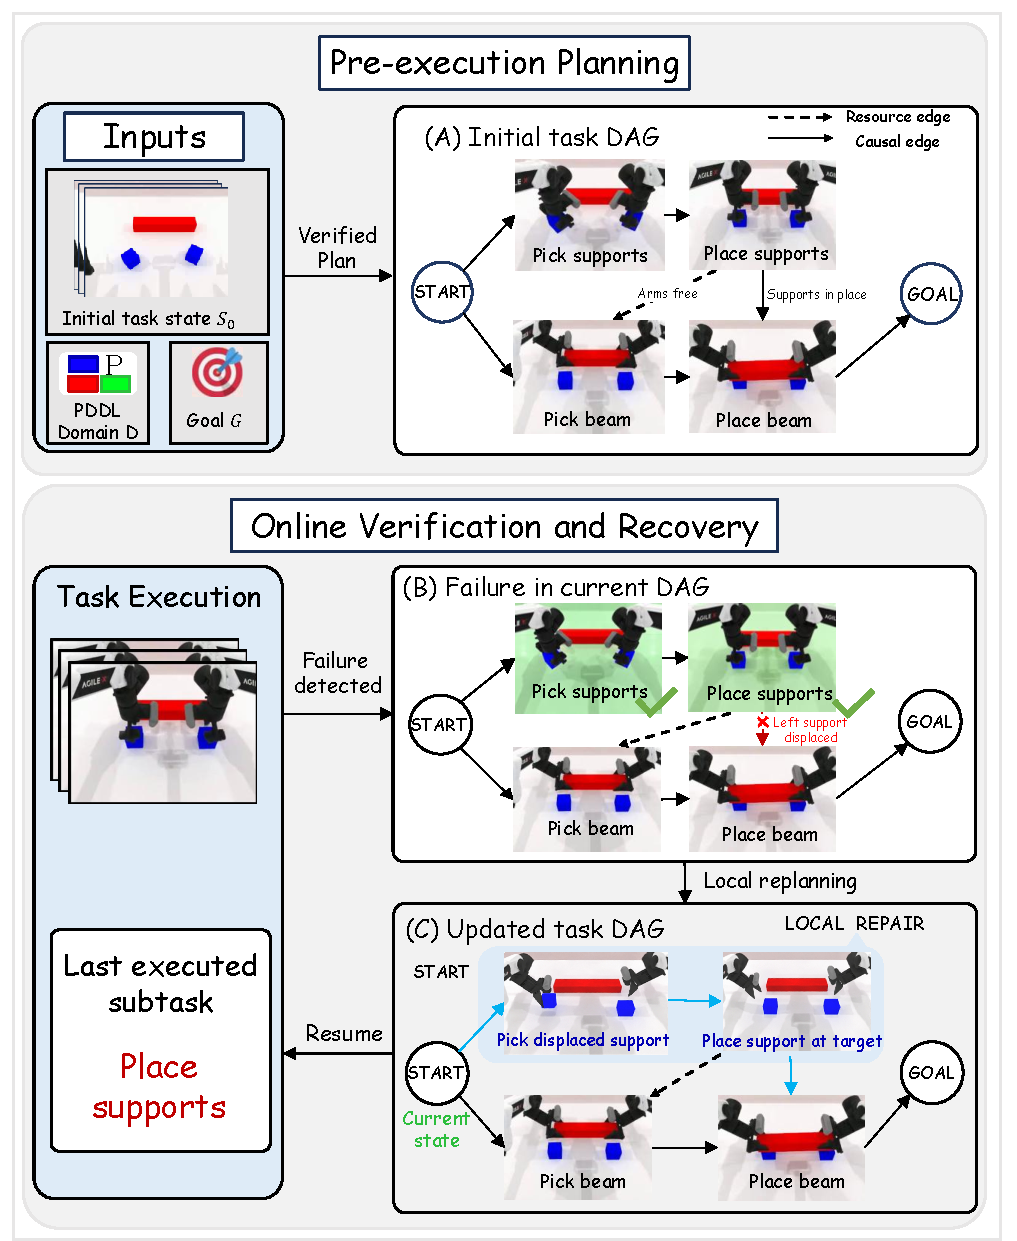
\includegraphics[width=\columnwidth]{Intro beautiful.pdf}
  \caption{\method execution on the BiCoord \texttt{build\_bridge} task.
  (A) A validated reference plan is compiled into the initial task DAG before execution.
  (B) A previously placed support is displaced, invalidating a condition required by the remaining plan.
  (C) \method repairs only the affected support operations, retains the unaffected beam operations, and resumes execution on the updated task DAG.}

  \label{fig:teaser}
\end{figure}

High-level planners follow two broad approaches. The first uses LLMs or VLMs to select skills, understand environmental feedback, determine action locations, and sequence the execution order of multi-step actions~\cite{ahn2024autort,ouyang2025long,huang2024rekep,feng2025reflective,chen2025robohorizon,ji2026hime,peng2026cortex,zhang2026harness,huang2026roboharness}. These methods can decompose tasks based on open instructions and respond to environmental changes, but typically generate only subgoals, text prompts, or short-term predictions, making it difficult to directly ensure the executability of a complete plan~\cite{yang2025guiding,chen2025code}. Alternatively, executable programs or symbolic formulations use classical planners, PDDL, or task-and-motion planning to generate constrained sequences~\cite{sakib2024consolidating,chen2024roboscript,yang2025guiding,kwon2025fast,chen2025code,chu2025llm+}. They check preconditions and constraints explicitly, but generally require a supplied symbolic state. Both classes of methods share a fundamental limitation: online recovery typically focuses on the step that has just failed or on the latest observation, without continuously tracking which action established each condition and which subsequent actions depend on it. When a visual fact changes or the effect of an earlier action is disrupted, the failure may surface several steps later, while its actual impact can extend to multiple actions that are not adjacent in the execution sequence.

Based on these observations, we introduce \method, a closed-loop framework above an existing low-level policy. As shown in Figure~\ref{fig:teaser}, \method consists of two stages: pre-execution planning and closed-loop execution. Each task type has an initial task graph, which may evolve differently depending on the disturbances encountered during execution. Before execution, \method generates a high-level action plan from the initial state and task goal. Once the plan passes logical validation, it is compiled into a task graph, where nodes represent executable subtasks and edges encode their dependencies. During execution, \method selects a ready action from the graph and checks its conditions before dispatching it to the low-level policy. After the action is completed, \method verifies its outcome and the dependencies required by subsequent actions. If a failure is confirmed, LOGIV identifies the affected branch, replans only that part of the graph, and preserves the remaining valid actions. The repaired plan is then validated, compiled into an updated task graph, and returned to the execution loop.

We evaluate \method on 20 simulated bimanual tasks from RoboTwin~V2 and BiCoord using $\pi_{0.5}$, AHA-WAM, and Light-WAM as backbones, together with real-robot experiments. Across the three backbones, \method improves mean success rate from 71.67\% to 82.33\% (RoboTwin~V2) and from 42.33\% to 57.67\% (BiCoord) under the situation of no disturbance. Under controlled execution-time perturbations, it also outperforms three matched corrective baselines. Our contributions are:
\begin{itemize}
  \setlength{\itemsep}{0pt}
  \setlength{\topsep}{2pt}
  \item We formulate dependency-aware recovery for long-horizon robot execution. The problem is to identify which future actions require repair and which completed results remain valid after a failure.
  \item We propose \method, which leverages task graphs to record conditional support, replans relevant branches along failure dependencies, and validates repair strategies while preserving valid work.
  \item Evaluations were conducted on 20 dual-arm tasks across RoboTwin V2 and BiCoord, using three different VLA/WAM backbones. LOGIV achieved state-of-the-art performance under a unified setting and demonstrated its effectiveness through real-robot experiments.
\end{itemize}

\section{Related Work}
\subsection{Long-Horizon Manipulation with VLA and WAM}
For long-horizon operations, existing work primarily enhances VLA and WAM at two levels: the execution organization and the base model. The first category of methods introduces high-level modules beyond the low-level policy. The low-level policy executes individual actions, while the high-level module selects and sequences them using current observations and task history. HiMe preserves context with hierarchical memory, Cortex unifies the VLM-planner and VLA-executor subtask interface, Harness VLA and RoboHarness use execution memory to select and connect policies~\cite{ji2026hime,peng2026cortex,zhang2026harness,huang2026roboharness}. Another category of methods directly improves VLA or WAM's modeling of task processes and environmental changes. RoboHorizon enables long-horizon planning using multi-stage rewards and a multi-perspective world model, Fast-WAM learns environment dynamics through video modeling during training while eliminating future generation at test time, and AHA-WAM enhances the efficiency of long-term information utilization via asynchronous world and action branches.~\cite{chen2025robohorizon,yuan2026fast,cai2026aha}. These approaches enhance the organization or generation of long-range tasks, but do not address how to repair affected steps and retain valid work when external disturbances cause earlier results to fail.

\subsection{Plan Verification and Recovery}

Recent work increasingly combines online visual feedback with structured plan representations for execution verification and recovery~\cite{ahmad2025unified}. VeriGraph uses scene graphs to validate and revise candidate action sequences~\cite{ekpo2024verigraph}, while related graph-based methods maintain online task information and execution structure~\cite{booker2024embodiedrag,shirasaka2025spark,yang2026integrated,zhang2026atomic}. Unlike explicit graph representations, LERa identifies and explains errors from the latest observation before revising the plan, Reflective Planning reassesses actions by predicting future images~\cite{pchelintsev2025lera,feng2025reflective}, and behavior trees switch to recovery branches when action conditions fail~\cite{colledanchise2016behavior,iovino2022survey}. These methods can detect errors and update plans, but they do not use action dependencies to determine the repair scope while preserving unaffected work.


\begin{figure}[!b]
  \centering
  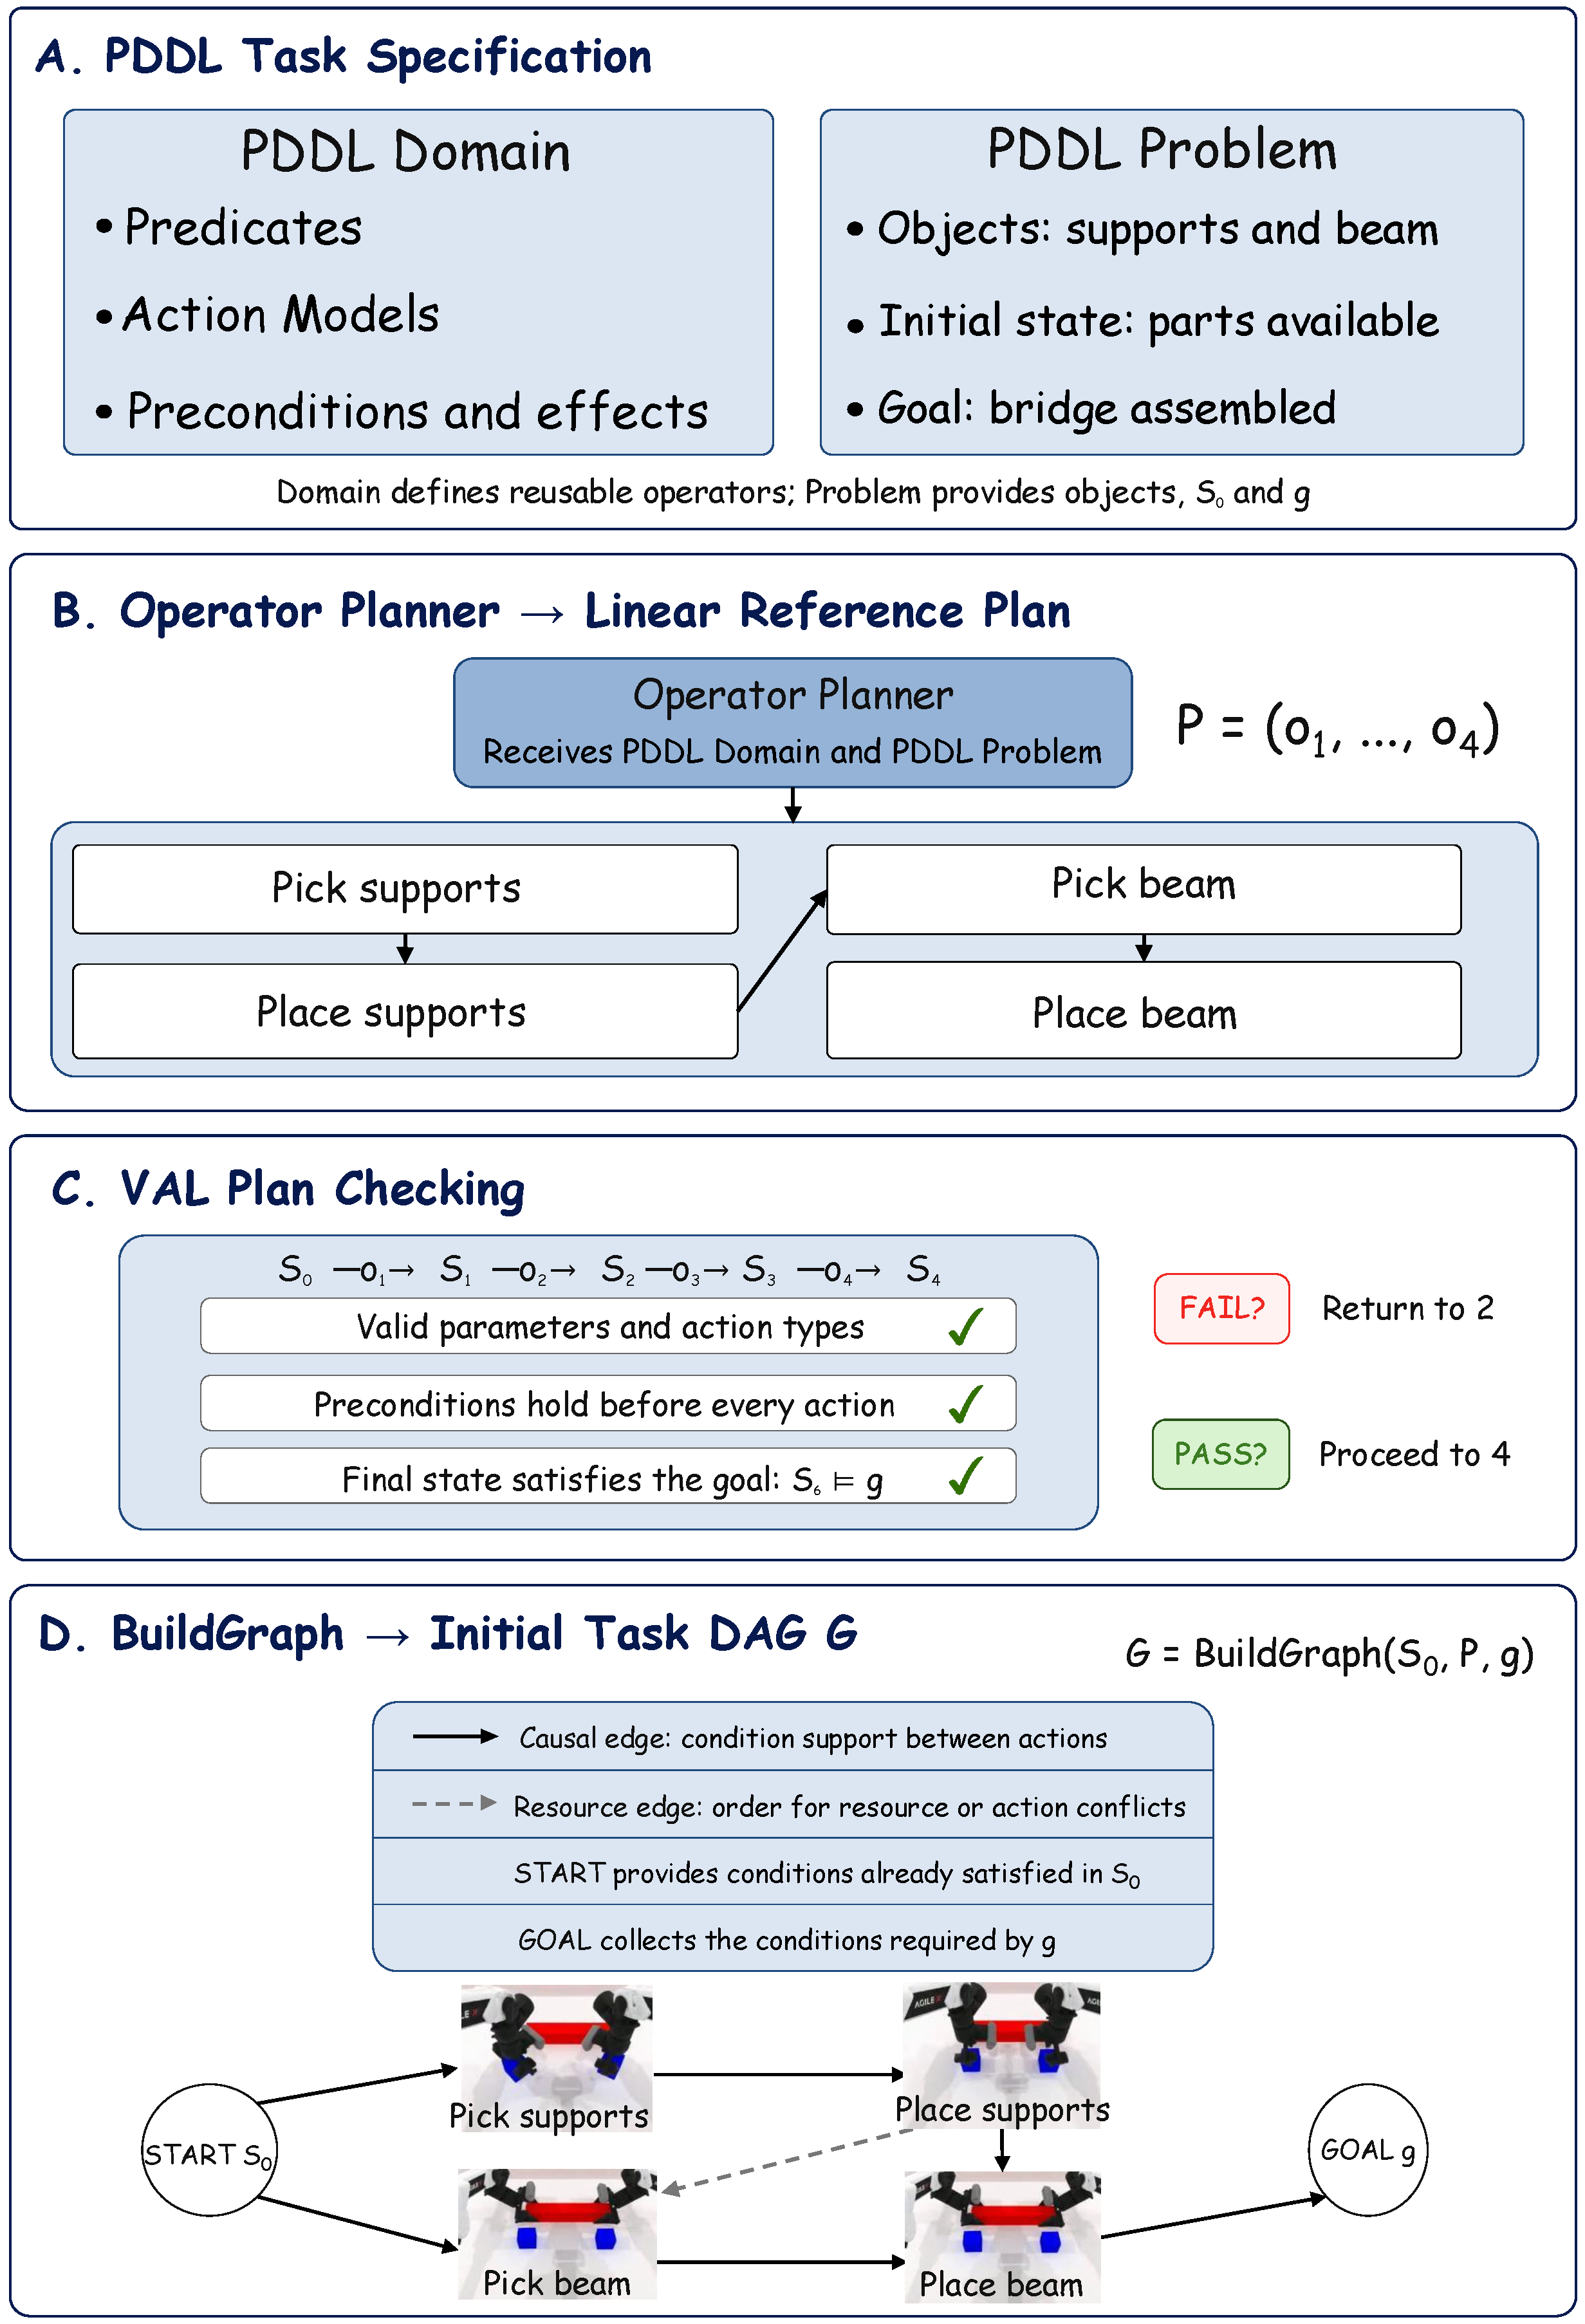
\includegraphics[width=0.94\columnwidth]{LOGIV_pre beautiful.pdf}
  \caption{\method pre-execution planning and task-graph construction. The Operator Planner generates reference plan $P$, where each $o_i$ in panel (B) is a grounded high-level PDDL operator. After validation by VAL, $P$ is compiled into the initial task graph $G$.}
  \label{fig:preplan}
\end{figure}

\section{Method}
\method is a closed-loop planning, verification, and local-repair framework that wraps an existing robot policy (VLA or WAM). The policy executes individual subtasks, while \method generates and monitors the plan, then repairs the affected conditions after an action failure or environmental change. Section~III-A first defines the research problem addressed in this paper, Section~III-B introduces pre-execution planning, verification, and task graph construction, Section~III-C presents online monitoring, local repair, and plan updating during execution.

\subsection{Problem Formulation}
We study high-level plan repair for long-horizon manipulation. \method builds an initial task graph $G$ before execution and advances it online from low-level-policy feedback.

At time $t$, $S_t$ is the latest reliable state derived from robot status, actuator feedback, and VLM's semantic conclusions parsed from visual observations $O_t$. Given initial state $S_0$ and goal $g$, the Operator Planner in Equation~\eqref{eq:plan} generates the reference plan $P=(o_1,\ldots,o_n)$. Each $o_i$ is a grounded high-level PDDL operator whose preconditions and effects are used for VAL checking~\cite{howey2004val} and graph construction~\cite{aeronautiques1998pddl}. Positions in $P$ define the reference order for compiling a directed acyclic task graph $G=(V,E)$. Here, $V$ contains subtask nodes, together with \textsc{start} and \textsc{goal}. In $E$, Causal edges encode precondition support and Resource edges constrain execution order. Together, these edges record which action supports each condition and which actions must remain ordered during execution.
\begin{align}
P&=\operatorname{PreparePlan}(S_0,g)=(o_1,\ldots,o_n), \nonumber\\
G&=(V,E)=\operatorname{BuildGraph}(S_0,P,g).
\label{eq:plan}
\end{align}
Execution is scheduled by task graph $G$, which identifies ready nodes from their dependencies and completion status. The selected subtask node is expressed as a natural-language instruction and passed with the visual observation to a low-level policy such as a VLA or WAM. After each subtask, \method{} derives the latest reliable state $S_{t+1}$ from observation $O_{t+1}$ and execution feedback, then updates the node completion status in $G$. Upon confirming a failure, it records error $e_t$. Based on $S_{t+1}$ and $e_t$, \method{} follows the Causal edges to identify the affected unfinished nodes. All other valid nodes are retained, while new high-level operators are generated only for the affected part. The new and retained operators together form the reference plan $P'$. After VAL validates $P'$, \method{} rebuilds the task graph $G'$ and selects a new ready node to resume execution. Equation~(2) summarizes the overall process.

\begin{equation}
(P',G')=\operatorname{TopologyGuidedRepair}(S_{t+1},e_t,P,G).
\end{equation}

\begin{algorithm}[t]
\algcaption{\method Task-Graph Execution and Topology-Guided Repair}
\label{alg:logiv}
\textbf{Require} initial task state $S_0$, task goal $g$\par
\textbf{Output} \textsc{success} or \textsc{failure}\par\vspace{2pt}\hrule
\begin{compactalgorithmic}
\item $P\leftarrow\operatorname{PreparePlan}(S_0,g)$
\item \textbf{if} $P=\textsc{fail}$ \textbf{then return} \textsc{failure}
\item $G\leftarrow\operatorname{BuildGraph}(S_0,P,g)$
\item $t\leftarrow 0$
\item \textbf{while} execution budget remains \textbf{do}
\item \hspace*{1.5em}$v\leftarrow$ next ready node in $G$ or \textsc{goal}
\item \hspace*{1.5em}$(\texttt{status},S_{t+1},e_t)
      \leftarrow\operatorname{VerifyAndExecute}(v,G,S_t)$
\item \hspace*{1.5em}\textbf{if} $\texttt{status}=\textsc{unresolved}$
      \textbf{then return} \textsc{failure}
\item \hspace*{1.5em}\textbf{else if} $\texttt{status}=\textsc{pass}$
      and $v=\textsc{goal}$ \textbf{then return} \textsc{success}
\item \hspace*{1.5em}\textbf{else if} $\texttt{status}=\textsc{pass}$ \textbf{then}
\item \hspace*{3em}set $v$ in $G$ to completed
\item \hspace*{1.5em}\textbf{else} \quad
      \algcomment{confirmed \textsc{fail}} 
\item \hspace*{3em}record $e_t$ and the failed condition on $v$ in $G$
\item \hspace*{3em}$(P',G')\leftarrow
      \operatorname{TopologyGuidedRepair}(S_{t+1},e_t,P,G)$
\item \hspace*{3em}\textbf{if} $P'=\textsc{fail}$
      \textbf{then return} \textsc{failure}
\item \hspace*{3em}$(P,G)\leftarrow(P',G')$
      \quad \algcomment{Update reference plan and task graph}
\item \hspace*{1.5em}\textbf{end if}
\item \hspace*{1.5em}$t\leftarrow t+1$
\item \textbf{end while}
\item \textbf{return} \textsc{failure}
\end{compactalgorithmic}
\end{algorithm}


\begin{figure*}[t]
  \centering
    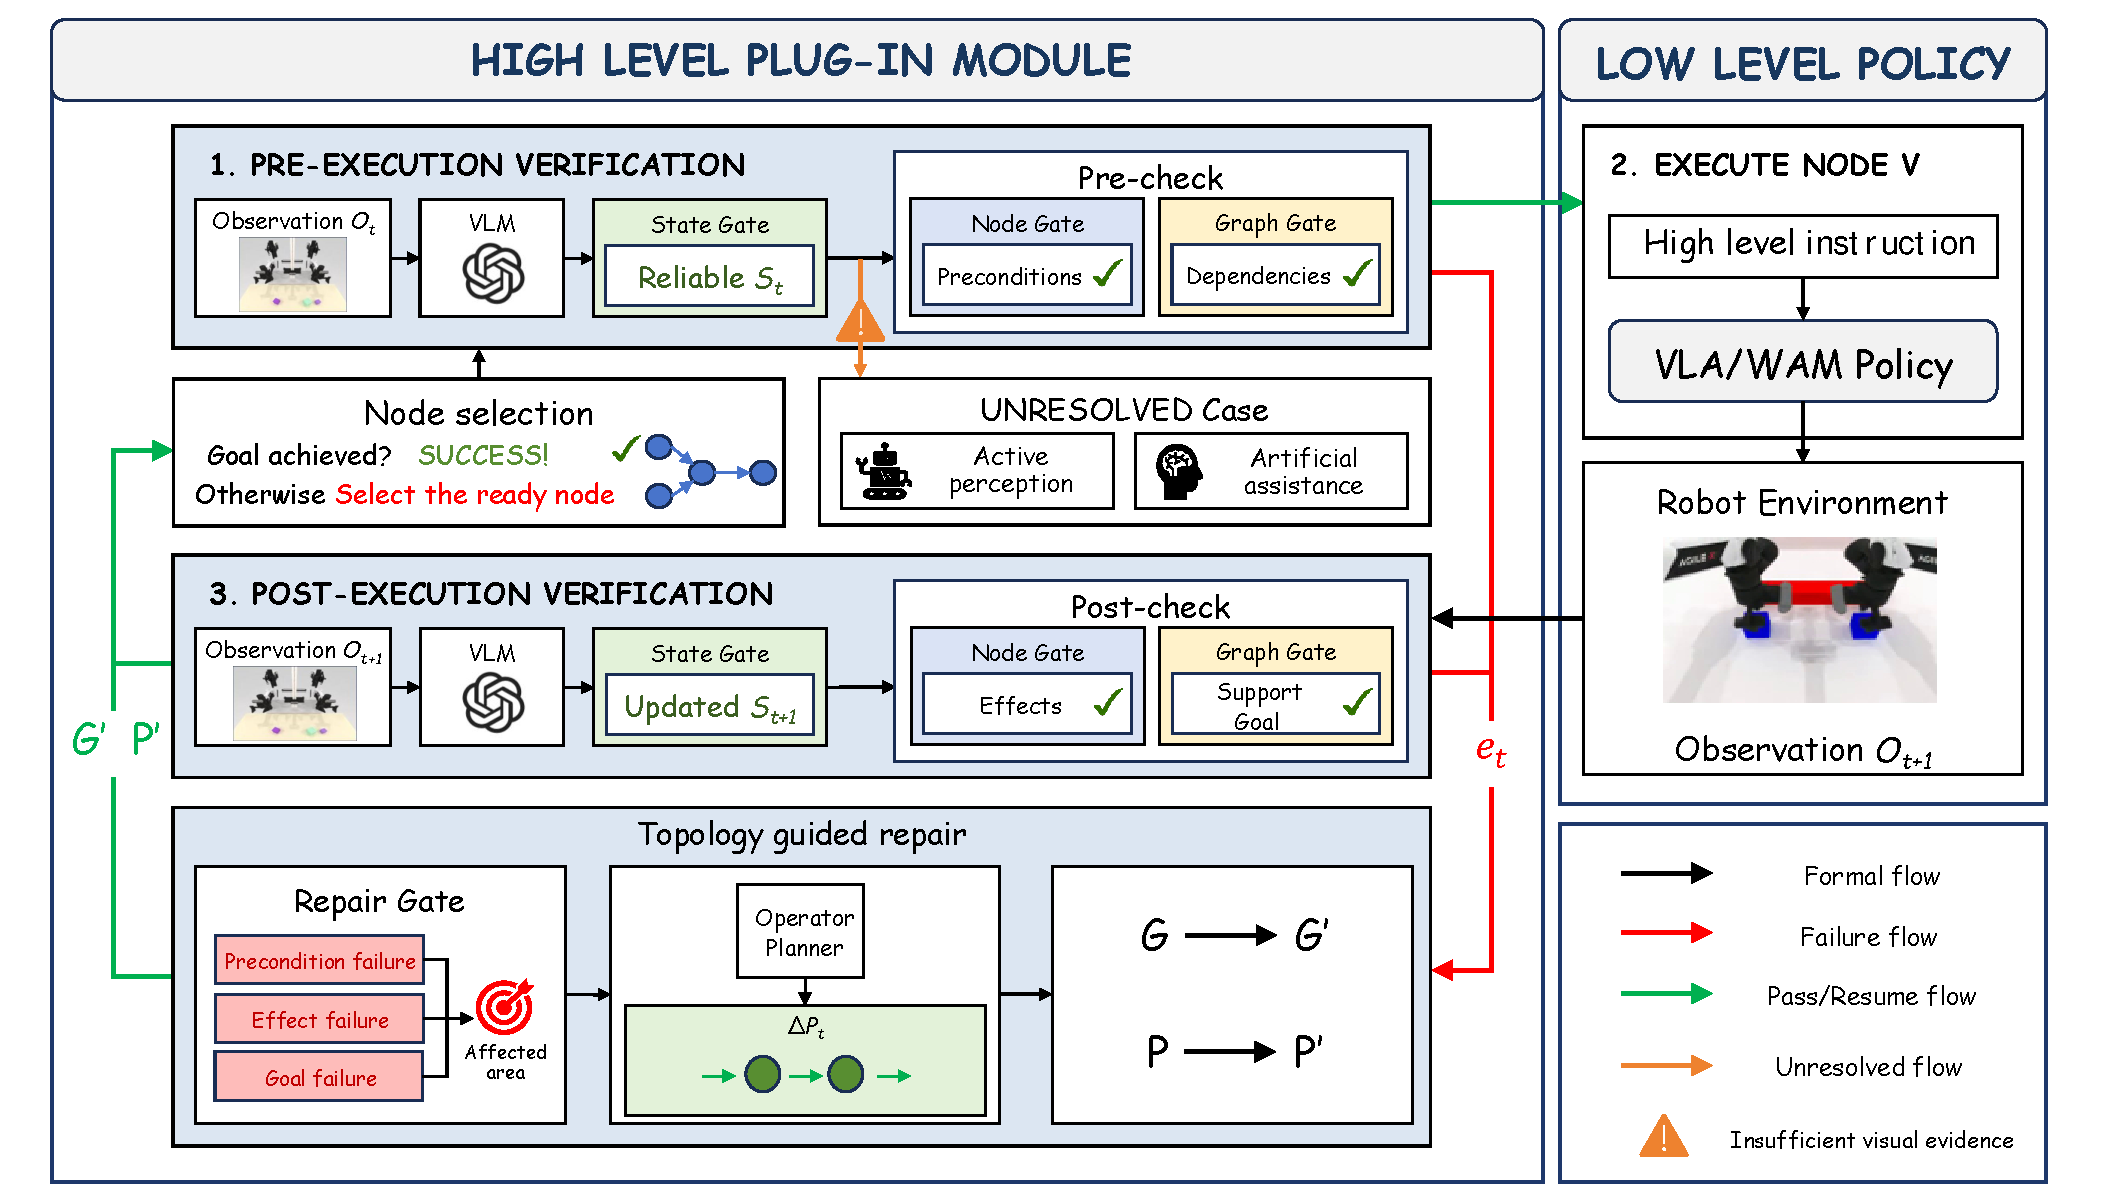
\includegraphics[width=\textwidth]{Method beautiful version cropped.pdf}
    \caption{\method online verification and topology-guided causal local repair. Three Gates establish reliable task facts, verify the selected subtask and graph dependencies. Upon a failure, the Repair Gate identifies affected nodes, validates a local repair plan, rebuilds the task graph, and resumes execution.}
  \label{fig:overview}
\end{figure*}

\subsection{Pre-Execution Planning}
\textbf{Plan generation and validation.}
To construct $P$, the Operator Planner takes the PDDL Domain and Problem shown in Figure~\ref{fig:preplan}(A). The Domain defines reusable operators, parameters, preconditions, and effects. The Problem specifies the objects, $S_0$, and $g$~\cite{aeronautiques1998pddl}. In Fig.~\ref{fig:preplan}(B), the planner binds high level operator to objects and runs LAMA-first~\cite{richter2010lama} in Fast Downward~\cite{helmert2006fast}. Starting from $S_0$, it repeatedly selects an operator whose preconditions hold, applies its effects to the simulated symbolic state, and derives the next state. This continues until the state satisfies $g$, yielding an executable order $P=(o_1,\ldots,o_n)$. After constructing support and order edges, $P$ is a topological order of $G$.

Figure~\ref{fig:preplan}(C) shows VAL independently replaying $P$ from $S_0$ under the planner's update rule. VAL checks the object bindings and preconditions of each $o_i$. If they pass, it applies the effects of $o_i$ and checks $o_{i+1}$ against the updated state. After replaying all operators, VAL checks whether the final state satisfies $g$~\cite{howey2004val}. On failure, VAL returns the first failing location and cause. The planner adjusts and replans until the complete plan $P$ passes validation, then graph construction begins.

\textbf{Task-graph construction.}
Figure~\ref{fig:preplan}(D) shows how \method compiles the validated reference plan $P$ into a directed acyclic task graph (DAG) $G$. Each operator in $P$ becomes a subtask node. The graph also contains \textsc{Start} and \textsc{Goal}. Causal edges represent condition support between nodes. Resource edges represent ordering constraints caused by resource use or action interference. In the initial task graph, \textsc{Start} provides conditions that already hold in $S_0$. The \textsc{Goal} node collects the conditions in task goal $g$. 

Then we consider the edges. For each precondition of operator $o_i$ in $P=(o_1,\ldots,o_n)$, the compiler searches the preceding operators in reverse order. It selects the nearest operator $o_j$ that establishes the condition without it being invalidated before $o_i$. The compiler then adds a Causal edge from $o_j$ to $o_i$ and records the supported condition on the edge. If no preceding operator establishes the condition and it already holds in $S_0$, the Causal edge starts from \textsc{Start}. The same procedure connects the last valid source of each goal condition to \textsc{Goal}. Resource edges preserve the order required for safe execution. They are added when two actions share an arm, gripper, or another exclusive resource. Their direction follows the relative order in $P$. Since both edge types follow $P$, the resulting graph remains acyclic and $P$ is one of its valid topological orders. The tuple $(P,G,S_0)$ is then passed to the online execution loop.




\subsection{Online Verification and Recovery}

\textbf{Task-graph scheduling and online checking.}
Figure~\ref{fig:overview} shows the online phase schedules high-level actions based on the task graph $G$. During the $t$-th execution round, the Node Selection module selects ready nodes according to dependencies and completion status within the graph. A subtask node becomes ready only if the conditions recorded by causal edges are satisfied in state $S_t$, and all preceding nodes specified by resource edges have been completed. When multiple nodes become ready simultaneously, the system selects the one with the earliest position in the reference plan $P$. Subsequently, the State Gate, Node Gate, and Graph Gate sequentially perform state information filtering, node execution validation, and graph-level dependency checks. Reliable information generated from these checks and executions is used to derive the next state $S_{t+1}$. If verification fails, the system records an error $e_t$ and triggers a recovery mechanism.

Before execution, the VLM parses relevant task facts from the visual observation $O_t$ based on the current high level operator's verification requirements. The State Gate fuses these facts with the robot's state and actuator feedback to form the current reliable state $S_t$. When visual evidence is insufficient, the robot actively perceives by acquiring new images, changing viewpoints, or rechecking the current node, or it may request human assistance. If confirmation remains unachievable within the budget, the system returns \textsc{UNRESOLVED} and halts the current execution. Subsequently, the Graph Gate checks whether prerequisite nodes specified by Resource edges have been completed and whether the supporting conditions defined by Causal edges still hold. For Causal edges originating from \textsc{START}, the Graph Gate verifies the conditions recorded on the edge. The Node Gate checks the preconditions of the action. If any check fails, the system does not execute the action and returns \textsc{FAIL}, marking $e_t$ as \texttt{PRECONDITION\_FAILURE}. Upon successful completion of both checks, the current high level operator is verbalized and passed to the low-level policy for execution.
After execution, the VLM parses observation $O_{t+1}$. The State Gate combines the new facts with proprioception and actuator feedback to produce the next reliable state $S_{t+1}$. The Node Gate checks whether the expected action effects hold. The Graph Gate checks whether conditions needed by the remaining plan are still valid. A missing effect or invalidated dependency returns \textsc{fail} and sets $e_t$ to \texttt{EFFECT\_FAILURE}. If both checks pass, the system returns \textsc{pass} and marks the current node as complete. Node Selection then selects the next node. When Node Selection reaches \textsc{Goal}, the system checks task goal $g$. If $g$ holds, execution returns \textsc{success}. Otherwise, the system returns \textsc{fail} and sets $e_t$ to \texttt{GOAL\_FAILURE}. Algorithm~\ref{alg:logiv} summarizes the checking and execution procedure as
\begin{equation}
\begin{aligned}
(\texttt{status},S_{t+1},e_t)
&=\operatorname{VerifyAndExecute}(v,G,S_t),\\
\texttt{status}
&\in\{\textsc{pass},\textsc{fail},\textsc{unresolved}\}
\end{aligned}
\label{eq:verify_execute}
\end{equation}
Here, $v$ is the node selected, the procedure receives reliable state $S_t$ and returns the latest reliable state as $S_{t+1}$. This output is defined even when the action is not executed because the pre-execution observations may update the reliable state. When no failure is confirmed, $e_t=\varnothing$.

\textbf{Repair scope and local replanning.}
The repair procedure first identifies the affected part of the task graph. In Algorithm~\ref{alg:logiv}, $\operatorname{TopologyGuidedRepair}$ receives the latest reliable state $S_{t+1}$, error category $e_t$, reference plan $P$, and task graph $G$. The failed node and related condition recorded in $G$ determine where the Repair Gate begins tracing. A \texttt{PRECONDITION\_FAILURE} starts from a missing precondition. An \texttt{EFFECT\_FAILURE} starts from a missing or invalidated effect. A \texttt{GOAL\_FAILURE} starts from an unsatisfied goal condition. The Repair Gate follows Causal edges to affected unfinished successors until no additional node depends on an invalidated condition. Resource edges do not expand this causal scope. They are reconsidered when the repaired task graph is constructed.

After determining the repair scope, the system collects the conditions required by retained downstream actions and the unsatisfied goal conditions previously supported by affected nodes. An invalidated effect of a completed action is also included when it is still required by the remaining plan. Other valid unfinished operators retain their original relative order. VAL first replays the retained operators before the repair position from $S_{t+1}$. The Operator Planner then generates a local operator sequence $\Delta P_t$ from the resulting state and inserts it between the retained parts. VAL checks whether the complete updated plan can execute from $S_{t+1}$ and reach goal $g$. A failure inside $\Delta P_t$ causes regeneration within the same scope. If a retained node remains infeasible, that node and its Causal-edge successors enter the next repair scope. If the final goal remains unsatisfied, the missing goal conditions are added to the next planning request. Repair stops when validation succeeds or the repair budget is exhausted.

The Operator Planner returns $\Delta P_t$ as a linear executable sequence rather than a fixed graph branch. After validation, \method combines it with the retained unfinished operators and rebuilds the remaining task graph using the construction rules in Section~III-B. Causal edges are recovered from condition support. Resource edges are added only where resource conflicts or action interference require an order. Therefore, adjacent operators in $\Delta P_t$ need not be directly connected in the rebuilt graph. The outgoing Causal edges of \textsc{Start} represent conditions already satisfied by the latest reliable state, including valid effects of completed actions. Completed nodes are not inserted into the remaining plan again. After the rebuilt graph is installed, Node Selection chooses the earliest ready node and online execution resumes.



\section{Experiments}
\subsection{Experiment Setup}
\textbf{Tasks.}
We evaluate \method on ten tasks from each of RoboTwin~V2~\cite{chen2025robotwin} and BiCoord~\cite{peng2026BiCoord} dual-arm simulators. Both natively support high-dimensional actions and coordinated dual-arm control, with multistage, cross-arm-dependent tasks suited to long-horizon verification and recovery. Table~\ref{tab:tasks} lists all 20 tasks. Each task has ten predefined initial states. Clean runs each state once without artificial perturbations. Perturbed reuses the same states and injects one recoverable disturbance at a predefined event. The disturbance type and trigger are fixed within a task but differ according to task goals and object relations. For example, in the task \texttt{move\_can\_pot}, the pot shifts laterally by 10 to 15\,cm after the can is grasped and lifted. 
\begin{table}[!t]
\centering
\caption{The 20 dual-arm tasks from RoboTwin~V2 and BiCoord.}
\label{tab:tasks}
\small
\renewcommand{\arraystretch}{1.05}
\setlength{\tabcolsep}{2pt}
\begin{tabular*}{\columnwidth}{@{\extracolsep{\fill}}ll@{}}
\toprule
\multicolumn{2}{c}{RoboTwin~V2~\cite{chen2025robotwin}} \\
\cmidrule(lr){1-2}
\texttt{beat\_block\_hammer} & \texttt{blocks\_ranking\_size} \\
\texttt{handover\_block} & \texttt{move\_can\_pot} \\
\texttt{open\_microwave} & \texttt{place\_dual\_shoes} \\
\texttt{stack\_blocks\_three} & \texttt{stack\_bowls\_three} \\
\texttt{stamp\_seal} & \texttt{turn\_switch} \\
\midrule
\multicolumn{2}{c}{BiCoord~\cite{peng2026BiCoord}} \\
\cmidrule(lr){1-2}
\texttt{cook} & \texttt{put\_objects\_cabinet} \\
\texttt{divide\_block\_tower} & \texttt{place\_plate\_and\_cup} \\
\texttt{build\_bridge} & \texttt{clean\_table} \\
\texttt{collect\_pens} & \texttt{match\_blocks\_with\_signs} \\
\texttt{jigsaw} & \texttt{exchange\_mics} \\
\bottomrule
\end{tabular*}
\end{table}

\textbf{Backbones and baselines.}
We use $\pi_{0.5}$, AHA-WAM, and Light-WAM as backbones. The $\pi_{0.5}$ backbone is a VLA execution policy~\cite{intelligence2025pi_}, while AHA-WAM and Light-WAM are based on world-action modeling~\cite{cai2026aha,li2026light}. On RoboTwin~V2, \method neither modifies nor retrains these backbones, while for BiCoord, task-specific fine-tuning was performed for the ten tasks. For each underlying execution model, we compare LOGIV with the backbone and three other state-of-the-art methods. \emph{VeriGraph-PDDL} retains the core idea of checking scene-graph constraints~\cite{ekpo2024verigraph} and replans the complete remaining task from reliable state $S_t$ when a constraint is violated. \emph{LERa-PDDL} uses visual feedback to analyze the failure cause, updates the planning conditions, and replans the complete remaining task from $S_t$~\cite{pchelintsev2025lera}. \emph{VLM-RP-BT} organizes the same initial plan as a behavior tree, generating and inserting recovery actions when a condition is unsatisfied~\cite{colledanchise2016behavior,iovino2022survey}. These baselines use a unified execution configuration to evaluate \method's performance relative to existing methods, ensuring a fair and reasonable comparison.

\textbf{Implementation details.}
We predefine the PDDL domain used in the experiments and keep it fixed across all experiments. Vision-language configurations use GPT-4o~\cite{hurst2024gpt} with at most 512 output tokens. Each node receives one pre-execution check and one post-execution check; \textsc{unresolved} permits at most three extra observations. Fast Downward uses LAMA-first with 30\,s per planning call and 5\,s per VAL validation. For each failure, the budget permits three local-repair rounds and four VLM calls; exceeding either ends the episode. Each $\text{Backbone}\times\text{Method}$ configuration runs 400 episodes with identical inputs, disturbances, success criteria, and computational budgets.

\textbf{Evaluation metrics.}
All backbones are trained or adapted using expert demonstrations without execution-time perturbations. We report the success rates of full-task completion both without artificial perturbations and after applying predefined perturbations. We also measure how often an invalidated condition is re-established within the given budget and passes the next relevant check. This measure includes only events that reach the injection point, successfully invalidate the designated condition, and remain recoverable using the existing action set. In the ablation study, we further examine the role of task topology in local repair by measuring the extent of plan modification and redundant execution. The former is the proportion of unexecuted nodes that are deleted, replaced, or replanned, while the latter counts still-valid completed actions unnecessarily executed again after repair. Lower values indicate more localized repair and less redundant execution.

\subsection{Detailed Results}
\begin{table}[!t]
\centering
\caption{\normalfont Performance of different backbones and online error correction methods.}
\label{tab:main}
\small
\renewcommand{\arraystretch}{1.03}
\setlength{\tabcolsep}{3.2pt}

\begin{tabular*}{\columnwidth}{@{\extracolsep{\fill}}llccc@{}}
\toprule
Backbone & Method & C $\uparrow$ & P $\uparrow$ & R $\uparrow$ \\
\midrule
\multicolumn{5}{c}{\textbf{RoboTwin~V2~\cite{chen2025robotwin}}} \\
\midrule
\multirow{5}{*}{$\pi_{0.5}$~\cite{intelligence2025pi_}}
& Backbone       & 56 & 32 & 18 \\
& VeriGraph-PDDL~\cite{ekpo2024verigraph} & 68 & 56 & 66 \\
& LERa-PDDL~\cite{pchelintsev2025lera}      & 67 & 57 & 64 \\
& VLM-RP-BT~\cite{colledanchise2016behavior,iovino2022survey}      & 63 & 58 & 68 \\
& \method       & \textbf{72} & \textbf{60} & \textbf{72} \\
\addlinespace[3pt]
\multirow{5}{*}{AHA-WAM~\cite{cai2026aha}}
& Backbone       & 85 & 60 & 35 \\
& VeriGraph-PDDL~\cite{ekpo2024verigraph} & 90 & 78 & 81 \\
& LERa-PDDL~\cite{pchelintsev2025lera}      & 88 & 79 & 82 \\
& VLM-RP-BT~\cite{colledanchise2016behavior,iovino2022survey}      & 91 & 80 & 80 \\
& \method       & \textbf{93} & \textbf{83} & \textbf{85} \\
\addlinespace[3pt]
\multirow{5}{*}{Light-WAM~\cite{li2026light}}
& Backbone       & 74 & 58 & 28 \\
& VeriGraph-PDDL~\cite{ekpo2024verigraph} & 76 & 68 & 65 \\
& LERa-PDDL~\cite{pchelintsev2025lera}      & 76 & 67 & 70 \\
& VLM-RP-BT~\cite{colledanchise2016behavior,iovino2022survey}      & 78 & 70 & 62 \\
& \method       & \textbf{82} & \textbf{72} & \textbf{79} \\
\midrule
\multicolumn{5}{c}{\textbf{BiCoord~\cite{peng2026BiCoord}}} \\
\midrule
\multirow{5}{*}{$\pi_{0.5}$~\cite{intelligence2025pi_}}
& Backbone       & 39 & 31 & 21 \\
& VeriGraph-PDDL~\cite{ekpo2024verigraph} & 46 & 39 & 56 \\
& LERa-PDDL~\cite{pchelintsev2025lera}      & 47 & 43 & 63 \\
& VLM-RP-BT~\cite{colledanchise2016behavior,iovino2022survey}      & 45 & 45 & 59 \\
& \method       & \textbf{50} & \textbf{48} & \textbf{68} \\
\addlinespace[3pt]
\multirow{5}{*}{AHA-WAM~\cite{cai2026aha}}
& Backbone       & 45 & 43 & 37 \\
& VeriGraph-PDDL~\cite{ekpo2024verigraph} & 56 & 46 & 77 \\
& LERa-PDDL~\cite{pchelintsev2025lera}      & 52 & 48 & 73 \\
& VLM-RP-BT~\cite{colledanchise2016behavior,iovino2022survey}      & 57 & 48 & 80 \\
& \method       & \textbf{62} & \textbf{53} & \textbf{84} \\
\addlinespace[3pt]
\multirow{5}{*}{Light-WAM~\cite{li2026light}}
& Backbone       & 43 & 39 & 31 \\
& VeriGraph-PDDL~\cite{ekpo2024verigraph} & 56 & 46 & 67 \\
& LERa-PDDL~\cite{pchelintsev2025lera}      & 51 & 45 & 65 \\
& VLM-RP-BT~\cite{colledanchise2016behavior,iovino2022survey}      & 58 & 43 & 68 \\
& \method       & \textbf{61} & \textbf{49} & \textbf{74} \\
\bottomrule
\end{tabular*}

\par\vspace{4pt}
\begin{minipage}{\columnwidth}
\normalfont\footnotesize
\raggedright
\textbf{C}: Task success rate without artificial perturbations;
\textbf{P}: Task success rate after applying predefined perturbations;
\textbf{R}: Recovery success rate for invalidated conditions
among valid, recoverable perturbation events.
All results are expressed as percentages (\%).
\end{minipage}
\end{table}


Table~\ref{tab:main} summarizes the overall results of \method on two benchmarks. Without artificial perturbations, the average task success rate of the three base models improved from 71.67\% to 82.33\% on RoboTwin V2 and from 42.33\% to 57.67\% on BiCoord after integrating LOGIV. Even in settings without human-induced disturbances, robots may still encounter naturally occurring state deviations and action failures, demonstrating that LOGIV is not limited to handling artificially injected perturbations but can also enhance task performance during normal execution. When predefined perturbations are introduced during execution, LOGIV still enables the robot to complete tasks more reliably. On RoboTwin V2, after integrating LOGIV, the task success rates of $\pi_{0.5}$, AHA-WAM, and Light-WAM reached 60\%, 83\%, and 72\%, respectively—representing improvements of 28, 23, and 14 percentage points compared to their pre-integration performance. On BiCoord, the success rates were 48\%, 53\%, and 49\%, respectively, up by 17, 10, and 10 percentage points. LOGIV outperformed all three correction baselines under both natural and induced perturbations, indicating its superior ability to support subsequent task execution even after external disruptions. We further examined whether disrupted conditions could be restored, and LOGIV demonstrated higher recovery success across all combinations of the two benchmarks and three base models compared to the three correction baselines. Overall, our method avoids focusing recovery solely on the current failure step, thereby preventing the omission of affected subsequent actions, and reduces unnecessary modifications to still-valid portions of the original plan during global replanning.

\subsection{Ablation Study}
\begin{figure}[!t]
  \centering
  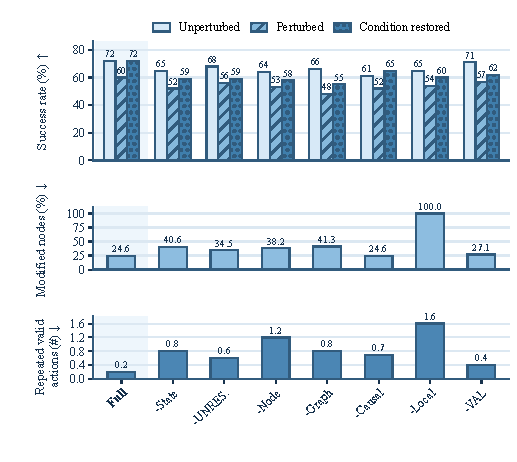
\includegraphics[width=\columnwidth]{ablation_bar_chart.pdf}
  \caption{Ablation results of LOGIV. Top panel reports task completion and condition restoration under perturbation settings. The middle and bottom panels show modified nodes and repeated valid actions during repair, respectively.
  Full: complete method; -State: no State Gate; -UNRES: no uncertainty handling; -Node: no Node Gate; -Graph: no Graph Gate; -Causal: no causal dependency tracing; -Local: replanning all remaining actions instead of local repair; -VAL: no logical validation of the repaired plan.}
  \label{fig:ablation}
\end{figure}

As shown in Fig.~4, we conduct ablation experiments from three aspects---execution verification, causal local repair, and logical validation of the repair plan---to analyze how LOGIV detects failures, identifies affected actions, and verifies repair outcomes. All variants in Fig.~4 use $\pi_{0.5}$ as the backbone, with identical visual inputs, VLMs, and planning budgets. Results show that reliable task execution requires trustworthy state assessment and continuous execution monitoring, together with dependency-based local repair and logical validation of the updated plan when failures occur.

\textbf{(1) Execution Verification and Uncertainty Handling.}
The State Gate, Node Gate, and Graph Gate respectively assess factual credibility, current actions, and subsequent dependencies; omitting any of these checks weakens both execution and recovery capabilities. Notably, skipping cross-action dependency checks leads to the lowest task success rate under perturbations. Forcing binary decisions when evidence is insufficient reduces the success rate of restoring invalidated conditions from 72\% to 59\%, highlighting the importance of preserving the \texttt{UNRESOLVED} state.
\textbf{(2) Graph Structure and Local Repair.}
After detecting a failure, accurately locating affected actions is essential. Selecting nodes solely based on their positions in the linear plan $P$ leaves the average repair scope unchanged but reduces task success without injected perturbations from 72\% to 61\%. Replanning all remaining actions also increases redundant execution of still-valid steps. These results indicate that effective repair requires causal dependencies to identify affected nodes and local replanning to preserve valid progress.
\textbf{(3) VAL Logical Validation.}
After generating a repair fragment, its compatibility with the remaining plan must be verified. Omitting this step reduces the success rate of restoring invalidated conditions from 72\% to 62\%. VAL checks the preconditions of subsequent actions and satisfaction of the final goal, providing feedback to guide replanning and establish consistency between the repair fragment and the preserved plan at the symbolic level.

Overall, the three Gates and the \texttt{UNRESOLVED} state provide reliable foundations for failure detection, while the task graph and local repair confine replanning to affected regions. VAL further supports error correction through logical checks and feedback. The ablation results support the complementary roles of these components: detecting failures reliably, repairing along actual dependencies, and verifying the repaired plan together improve long-horizon task completion and recovery.


\subsection{Real-World Experiments}


\section{Conclusion}
This paper addresses a fundamental challenge in long-horizon robot execution: how to identify the parts that truly need re-execution when initial action conditions become invalid, while preserving valid outcomes. \method builds on a topological graph structure and employs a two-phase approach—pre-execution mapping and in-execution graph maintenance—to continuously monitor conditional dependencies among actions, track affected nodes, and update local plans accordingly. Experiments with RoboTwin~V2, BiCoord, and real robots demonstrate that this method improves task completion and disturbance recovery across different VLA/WAM backbones. More importantly, long-horizon reliability does not solely depend on larger end-to-end models. Maintaining a verifiable and updatable planning structure beyond existing strategies offers a practical way to handle execution errors and environmental changes without retraining. In the future, we will explore goal changes and incomplete states in open environments, and extend \method to multi-robot collaboration.

\FloatBarrier
\balance
\bibliographystyle{IEEEtran}
\bibliography{references}
\end{document}
